\chapter{Introducción}\label{chapter:introduction}
\addcontentsline{toc}{chapter}{Introducción}
El manejo de información geográfica ha sido de gran importancia a lo largo de la
historia en diversas áreas del conocimiento, y los mapas han sido la herramienta
fundamental para su representación. Inicialmente, su elaboración era artesanal, lo
que limitaba su calidad y distribución. Con la aparición de instrumentos como la
brújula y la imprenta, la fabricación de mapas ganó precisión y mayor accesibilidad.
Posteriormente, la revolución digital, junto con herramientas como escáneres e
impresoras, facilitó su expansión y difusión.
Luego, a partir del avance en la industria del software, se impulsó el desarrollo de
los Sistemas de Información Geográfica(SIG)\cite{SIG}, herramientas que permiten
organizar, almacenar, manipular y analizar grandes volúmenes de datos
georreferenciados. Estos sistemas integran factores socioeconómicos y
ambientales, facilitando la toma de decisiones en diferentes ámbitos. Con la llegada
del internet y las tecnologías móviles, se globalizó el acceso a aplicaciones
cartográficas, ampliando su uso en diversos sectores.
Con la afluencia de condiciones como el incremento en la capacidad de cómputo en
los teléfonos inteligentes, el desarrollo de plataformas eficientes de desarrollo de
software, el incremento de la velocidad de Internet y la nueva disponibilidad de
servicios de mapas de terceros, las aplicaciones cartográficas destinadas a la
recolección de información en sitios de interés mediante el uso de formularios, han
pasado a representar una herramienta esencial para el trabajo de campo en
diversas disciplinas. Su principal utilidad radica en la posibilidad de recopilar datos
en ubicaciones fuera del entorno habitual de oficina, siendo particularmente
relevantes en sectores como la ingeniería, la arquitectura y las ciencias sociales.
Estas aplicaciones no solo optimizan el proceso de captura de información, sino que
también garantizan la portabilidad y seguridad de los datos hasta su procesamiento
final.
Existen diversos escenarios donde la implementación de estas herramientas resulta
crucial. Por ejemplo, en el sector eléctrico, permiten gestionar información sobre el
estado de torres eléctricas en una ciudad para planificar su mantenimiento. En la
industria petrolera, facilitan el estudio de áreas potenciales para la expansión de
explotaciones. Asimismo, en las empresas de suministro de agua, estas
aplicaciones contribuyen a la identificación y priorización de reparaciones según la
gravedad de las roturas detectadas. Además, las entidades responsables del
saneamiento urbano pueden utilizarlas para monitorear la situación de los
vertederos y contenedores de basura.
Adicionalmente, estas aplicaciones tienen un papel significativo en la administración
pública, facilitando procesos como la recaudación de impuestos, la fiscalización de
normativas y la realización de cuestionarios en el ámbito gubernamental provincial.
El impacto de estas herramientas en el desarrollo social y en otros sectores es
considerable, lo que resalta la importancia de su estudio y continuo
perfeccionamiento para optimizar su aplicación en escenarios cada vez más
exigentes y diversos.
Este trabajo se centra en el desarrollo de aplicaciones móviles para la recolección
de datos georreferenciados mediante formularios, concluyendo con la
implementación de una aplicación que permitirá mejorar la eficiencia en el registro y
análisis de información geográfica.
\section{Motivación y Justificación}
La Casa del Software de la Facultad de Matemática y Computación (MatCom) de la
Universidad de La Habana (UH) tiene experiencia en el desarrollo de SIG,
destacándose el sistema OpenLatino GIS, que permite mostrar regiones y ofrece
herramientas para manipular datos geográficos. Anteriormente se trabajó con
Asistentes Digitales Personales (PDA\cite{PDA}), pero con el avance de la tecnología móvil,
en 2021 se comenzó a explorar el desarrollo para teléfonos inteligentes,
incursionándose así en el desarrollo de varias aplicaciones como Geobase\cite{geoBase},
Notificador/Encuestador\cite{notificadorEncuestador} y NetTopologic\cite{netTopologic}.
De manera paralela en la alcaldía de Managua, Nicaragua existe un sistema de
encuestas para una recogida de información sobre determinadas propiedades. La
importancia de estas encuestas radica en que con ellas se logran obtener los datos
necesarios para computar el valor de las propiedades, permitiéndole así a la alcaldía
cobrar los impuestos sobre las mismas. Al mismo tiempo, estas encuestas se
realizan de manera manual siendo completadas mediante formularios impresos en
papel. Por ende, surge la necesidad de automatizar, digitalizar y por ende facilitar el
proceso de recogida de la información sobre estas propiedades o predios mediante
una aplicación para dispositivos móviles, permitiendo ahorrar recursos físicos por
parte de las entidades encargadas.
Luego, se cuenta con la capacidad para el desarrollo de la propuesta de solución
dadas las habilidades técnicas adquiridas durante la carrera de Ciencias de la
Computación, además de la abundante bibliografía que hay sobre la plataforma de
desarrollo sobre la cual se desarrollará la aplicación(Flutter) y que la facultad cuenta
con experiencia en el desarrollo de aplicaciones similares con esta tecnología como
Geobase, Notificador, Encuestador y NetTopologic.

\section{Formulación del problema}
Por el convenio Cadic-Uh que se desarrolla en la Casa del Software de la facultad
MatCom de la Universidad de la Habana (UH), se presentó la tarea de desarrollar
una aplicación móvil llamada “Inventario” para la empresa Cadic-Nicaragua.
La aplicación Inventario para el censo de información predial, es una herramienta
para el sistema operativo Android, que tiene como funcionalidad principal permitir la
recolección de datos de interés de un conjunto de edificaciones y predios(porciones
de terreno), mediante un mapa que muestra el área territorial a censar y las
divisiones entre predios. Esta tiene como objetivo ser usada por las alcaldías, que
realizan el proceso de censo una vez al año con el propósito de percibir ingresos a
través de la recaudación de tributos aplicados a las entidades responsables de cada
predio o edificación y por ende debe permitir el levantamiento por campos o
módulos a través de formularios, campos los cuales son concebidos a continuación:
Cada predio tendrá 5 módulos(campos) a rellenar, los cuales describirán o valorarán
el estado de los edificios y recolectarán información del terreno:
\begin{itemize}
    \item[$\rightarrow$] Edificación: Valora el estado del edificio, desde un antejardín hasta el
          estado de canoas bajantes.
    \item[$\rightarrow$] Terreno: Permite recolectar información del predio, como niveles del predio,
          el tipo de acera, el ancho de acera, etc.
    \item[$\rightarrow$] Construcción: Permite valorar el estado actual de los inmuebles en un
          predio.
    \item[$\rightarrow$] Uso de suelo y patentes comerciales: Información de importancia de la o
          las actividades económicas que se encuentren en un edificio.
    \item[$\rightarrow$] Medidores eléctricos: Información acerca de los medidores eléctricos que
          posee cada edificio en un predio.
\end{itemize}
Esta aplicación debe cumplir con los siguientes requerimientos funcionales, no
funcionales y de entorno:
\begin{itemize}
    \item Debe correr sobre el sistema Android. Teniendo compatibilidad con versiones
          anteriores a la versión 10.0.
    \item Interfaz de usuario sencilla y amigable.
    \item Deben soportar un visor de mapas que consuma una cartografía sin conexión
          a Internet.
    \item Tiene que consumir de un servicio externo la cartografía y las propiedades
          con la información que hay que mostrar.
    \item El mapa estará dividido en manzanas, las manzanas en predios, y los predios
          en edificios. Los colores a emplear para enmarcar las divisiones serán: verde,
          rojo y negro respectivamente.
    \item Cada manzana posee un número único.
    \item Debe permitir crear, modificar y eliminar mediante formularios, los 5 módulos
          mencionados.
    \item Compatibilidad con un futuro software de sincronización de datos, que
          mantendrá los campos o módulos rellenados por cada consultor,
          centralizados en una misma base de datos a nivel de empresa.
    \item Acceso al recorrido óptimo entre predios; dada una lista de predios a visitar,
          la localización actual del consultor y una relación de distancias entre los
          predios, ya sea la euclidiana o una relación de distancias vectorial como en
          para un óptimo más real.
    \item Posibilidad de guardar un registro con previas modificaciones a los módulos,
          en cada uno de los predios.
    \item Como se muestra en la figura 1, cada predio deberá tener un número de
          localización que se estructura de la forma: No. parcela + No. manzana + No.
          distrito:
          \begin{figure}[h]
              \centering
              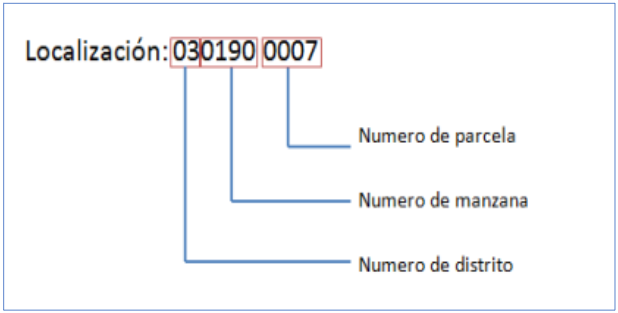
\includegraphics[scale=0.5]{Graphics/1.png}
              \caption{Figura 1: Descripción y delimitación del número de localización de un predio.} % Título de la figura
              \label{fig:figura1}
          \end{figure}
\end{itemize}
Por ende el problema de este trabajo puede ser enunciado como la carencia de una
aplicación móvil que permita automatizar el proceso de encuesta a propiedades y
recogida de información mediante formularios, que además cumpla con los
requerimientos funcionales, no funcionales y de entorno planteados anteriormente.
Dando paso a la siguiente pregunta científica:
\textbf{¿Será posible desarrollar una aplicación móvil que cumpla con los requerimientos
    planteados en este epígrafe y así dar solución al problema planteado?}




\section{Objetivos generales y específicos}
Como objetivo general se tendrá desarrollar una aplicación que permita a los
encuestadores auditar los predios mediante el uso de formularios que permitan
recoger información sobre dichos predios, caracterizando los mismos en base a los
cinco módulos: Edificación, Terreno, Construcción, Uso de Patentes/Licencias
Comerciales y Medidores eléctricos; y además agregue funcionalidades como
podrían ser optimizar el camino que debe recorrer el consultor para visitar los
predios que le fueron asignados. De aquí se derivan varios objetivos específicos o
parciales:
\begin{itemize}
    \item Investigar las distintas plataformas para el desarrollo de aplicaciones móviles.
          Ventajas y desventajas.
    \item Analizar las herramientas existentes para el trabajo con mapas en
          concordancia con el entorno de desarrollo seleccionado y que permita
          visualizar cartografía offline.
    \item Diseñar una arquitectura extensible, haciendo uso de los principios del
          desarrollo SOLID1 y empleando las buenas prácticas.
    \item Brindar mecanismos de acceso a los sensores del dispositivo móvil para una
          recopilación de datos más completa, dígase GPS2
          , cámara, como los
          principales.
    \item Cumplir con los requerimientos de las aplicaciones móviles pedidos por el
          cliente.
\end{itemize}

\section{Estructura del trabajo}
Este trabajo está compuesto por cuatro capítulos estructurados de la siguiente
manera:
\begin{itemize}
    \item Capítulo I: El primer capítulo presenta una breve introducción al tema, la
          motivación y justificación del mismo, la formulación del problema y los objetivos
          principales, concluyendo este capítulo con la estructura del trabajo.
          2 Sistema que permite posicionar cualquier objeto sobre la Tierra con una precisión de hasta
          centímetros, aunque lo común son unos pocos metros.
          1 Acrónimo que agrupa 5 principios clave para el desarrollo eficiente, replicable, mantenible y
          escalable de software.
    \item Capítulo II: Acá se analizan diferentes sistemas que ofrecen funcionalidades
          similares a la propuesta a desarrollar con el objetivo de explicar sus ventajas y
          desventajas. Se analizan además diferentes plataformas para el desarrollo de
          aplicaciones móviles y algunas tecnologías para el trabajo cartográfico.
    \item Capítulo III: Se verifica de una manera teórico-computacional la propuesta de
          solución. Además se dan algunos detalles de implementación que se consideran
          atractivos de explicar.
    \item Capítulo IV: En este capítulo se muestra el correcto funcionamiento del software
          creado y el cumplimiento de los objetivos del trabajo, con varias pruebas que se le
          hacen a la aplicación y a las distintas herramientas implementadas. Por último
          contamos con las conclusiones y recomendaciones de esta tesis.
\end{itemize}

